\section{Data}

Our data sets need to be preprocessed in order to apply a customary machine learning pipeline.
The data preprocessing should be generalizable to different regions, data formats, data types (vector vs.\ raster), coordinate systems, and so on.
This will allow any potential models to be trained and/or tested against other geographic regions.

The data sets represents data over a continuous geographic area.
We must therefore define a \textit{sample space} which allows us to split the data into respective training, validation, and test sets.
Our sample space will be the respective cadastral plots defined over a given region.
The intent is to implement an algorithm which receives the geographic extent of a cadastral plot and returns a segmentation map of the buildings within the provided area.

The preprocessing is somewhat time- and space-consuming, and must therefore be performed before training and persisted to disk.
Finally, there is an intent to prevent any data loss during the preprocessing step, such as downsampling and interpolation, thus keeping the original raw features.
This allows us to experiment with different data augmentation techniques during training instead without having to preprocess the entire data set anew.


\subsection{Coordinate Systems}
The most common spherical coordinate system for representing \textit{arbitrary} positions on earth's surface is the \textit{geographic coordinate system} (GPS).
A given point, $\vec{p} = (\phi, \lambda, z)$, is represented by an angular latitude and longitude, $\phi$ and $\lambda$ respectively, and a radial distance from the mean sea level, $z$.
Negative values for $z$ do not necessarily imply that the given point is below the ground, as certain areas (such as in the Netherlands) are situated below sea level.
It is therefore not sufficient to represent elevation data with unsigned floating point numbers.

Even though GPS is able to uniquely represent geographic positions with a high degree of accuracy, it is unsuitable for many applications.
Cartesian transformations and norms are cumbersome to calculate, and data structures and visualizations which are fundamentally two dimensional, such as maps, rasters, and matrices, become difficult to with spherical coordinates.

In order to solve this problem we define a set of coordinate system \textit{projections} which approximate given regions of the earth's surface as flat planes.
The resulting coordinate systems are Cartesian, and thus allow us to represent geographic points in the more common $\vec{p} = (x, y, z)$ format.
Cartesian distance norms such as $||\vec{p}_1 - \vec{p}_2||_2$ and Cartesian translations $\vec{p}_1 + \vec{\Delta}$ stay within pre-defined error tolerances as long as operations are contained to the validity region of the given projection.

\begin{wrapfigure}[15]{r}{0.38\linewidth}
  \vspace{-1em}
  \centering
  \includegraphics[width=0.9\linewidth]{europe-utm-zones.png}
  \caption{
    \\
    The figure shows the UTM zones required in order to cover the entirety of Europe, from \texttt{29S} to \texttt{38W}.
    This public domain image has been sourced from Wikimedia~\cite{wiki:europe_utm_zones}.
  }%
  \label{fig:europe-utm-zones}
\end{wrapfigure}

One such Cartesian approximation of the earth's surface is the Universal Transverse Mercator (UTM) coordinate system which divides the earth into 60 rectangular zones. The UTM zones covering Europe are shown in~\figref{fig:europe-utm-zones}.
We will therefore exclusively use UTM zone \texttt{32V} for our datasets sourced from Trondheim, Norway, situated in the southern part of Norway.
Data in alternative coordinate systems will be transformed to this UTM zone before we start using the data.
Since this is an affine coordinate system, we can easily generalize any models to other coordinate systems by applying the correct affine transformations.

\texttt{GDAL} can be used to transform data between coordinate systems, e.g.\ converting from GPS to UTM \texttt{32V}:
\begin{shellcode}
$ gdaltransform \
    -s_srs EPSG:25830 \
    -t_srs EPSG:25830 ${source_data}
\end{shellcode}


\subsection{Data types}

Geographical data can largely be divided into two sub-categories, \textit{vector data} and \textit{raster data}.
We will give a brief overview of these two data representations.

\subsection{Vector data}

\begin{figure}[htb]
  \centering
  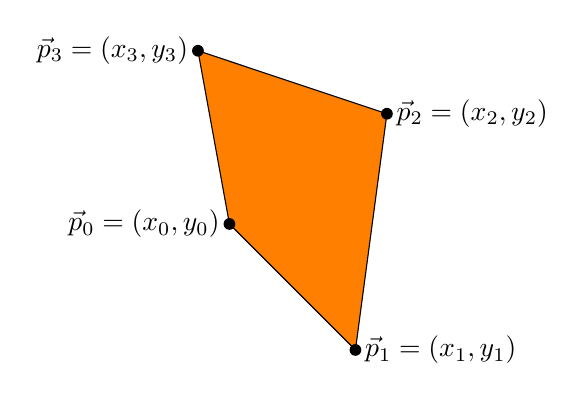
\begin{tikzpicture}[scale=2]
  \coordinate (zero) at (0, 0);
  \coordinate (one) at (0.8, -0.8);
  \coordinate (two) at (1, 0.7);
  \coordinate (three) at (-0.2, 1.1);
  \draw[fill=orange]
    (zero) node[left] {$\vec{p}_0 = (x_0, y_0)$}
    -- (one) node[right] {$\vec{p}_1 = (x_1, y_1)$}
    -- (two) node[right] {$\vec{p}_2 = (x_2, y_2)$}
    -- (three) node[left] {$\vec{p}_3 = (x_3, y_3)$}
    -- cycle;
  \foreach \n in {zero,one,two,three}
    \node at (\n)[circle,fill,inner sep=1.5pt]{};
\end{tikzpicture}

  \textcolor{gray}{\vrule}
  \hspace{0.01\linewidth}
  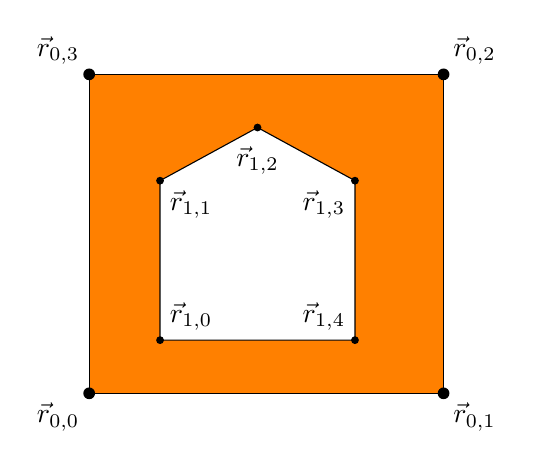
\begin{tikzpicture}[scale=2.25]
  \coordinate (zero) at (0, 0);
  \coordinate (one) at (2.0, 0);
  \coordinate (two) at (2.0, 1.8);
  \coordinate (three) at (0, 1.8);
  \draw[fill=orange]
    (zero) node[below left] {$\vec{r}_{0,0}$}
    -- (one) node[below right] {$\vec{r}_{0,1}$}
    -- (two) node[above right] {$\vec{r}_{0,2}$}
    -- (three) node[above left] {$\vec{r}_{0,3}$}
    -- cycle;
  \foreach \n in {zero,one,two,three}
    \node at (\n)[circle,fill,inner sep=1.5pt]{};

  \coordinate (0) at (0.4, 0.3);
  \coordinate (1) at (1.5, 0.3);
  \coordinate (2) at (1.5, 1.2);
  \coordinate (3) at (0.95, 1.5);
  \coordinate (4) at (0.4, 1.2);
  \draw[fill=white]
    (0) node[above right] {$\vec{r}_{1,0}$}
    -- (1) node[above left] {$\vec{r}_{1,4}$}
    -- (2) node[below left] {$\vec{r}_{1,3}$}
    -- (3) node[below=3.5pt] {$\vec{r}_{1,2}$}
    -- (4) node[below right] {$\vec{r}_{1,1}$}
    -- cycle;
  \foreach \n in {0,1,2,3,4}
    \node at (\n)[circle,fill,inner sep=1pt]{};
\end{tikzpicture}

  \caption{
    Simple polygon with four unique vertices is shown on the left hand side.
    A complex polygon with an an outer hull
    and an interior hull is shown on the right hand side for comparison.
  }
\end{figure}

\begin{figure}[H]
  \centering
  \begin{tikzpicture}[scale=1]
  \coordinate (ll) at (0, 0);
  \coordinate (mid) at (2, 1);
  \coordinate (lr) at (4, 0);
  \coordinate (ur) at (4, 2);
  \coordinate (ul) at (0, 2);
  \draw[fill=orange]
    (ll) node[left] {$\vec{r}_0$}
    -- (ur) node[right] {$\vec{r}_1$}
    -- (lr) node[right] {$\vec{r}_2$}
    -- (ul) node[left] {$\vec{r}_3$}
    -- cycle;
  \foreach \n in {ll,ur,lr,ul}
    \node at (\n)[circle,fill,inner sep=1.5pt]{};

   \draw (4.4, 1) edge[->, thick] node[above] {\texttt{buffer(0.0)}} (6.6, 1);

  \coordinate (offset) at (7, 0);
  \draw[fill=orange]
    ($ (ll) + (offset) $) node[left] {$\vec{r}_0$}
    -- ($ (mid) + (offset) $) node[below] {$\vec{r}_1$}
    -- ($ (lr) + (offset) $) node[right] {$\vec{r}_2$}
    -- ($ (ur) + (offset) $) node[right] {$\vec{r}_3$}
    -- ($ (mid) + (offset) $) node[above] {$\vec{r}_4$}
    -- ($ (ul) + (offset) $) node[left] {$\vec{r}_5$}
    -- cycle;
  \foreach \n in {ll,mid,lr,ur,mid,ul}
    \node at ($ (\n) + (offset) $)[circle,fill,inner sep=1.5pt]{};
\end{tikzpicture}

  \caption{Zero-buffering the polygon fixes self-intersecting polygons, as is shown here.}
\end{figure}

\begin{figure}[H]
  \centering
  \begin{tikzpicture}[scale=1]
  \coordinate (ll) at (0, 0);
  \coordinate (lm) at (2, 0);
  \coordinate (lr) at (4, 0);
  \coordinate (ur) at (4, 1);
  \coordinate (um) at (2, 1);
  \coordinate (Um) at (2, 2);
  \coordinate (ul) at (0, 1);
  \draw[fill=orange]
    (ll) node[below] {$\vec{r}_0$}
    -- (lm) node[below] {$\vec{r}_1$}
    -- (lr) node[below] {$\vec{r}_2$}
    -- (ur) node[above] {$\vec{r}_3$}
    -- (um) node[above right] {$\vec{r}_4$}
    -- (Um) node[above] {$\vec{r}_5$}
    -- (um) node[above left] {$\vec{r}_6$}
    -- (ul) node[above] {$\vec{r}_7$}
    -- cycle;
  \foreach \n in {ll,lm,lr,ur,um,Um,um,ul}
    \node at (\n)[circle,fill,inner sep=1.5pt]{};

   \draw (4.9, 0.5) edge[->, thick] node[above] {\texttt{buffer(0.0)}} (7.1, 0.5);

  \coordinate (offset) at (8, 0);
  \draw[fill=orange]
    ($ (ll) + (offset) $) node[below] {$\vec{r}_0$}
    -- ($ (lr) + (offset) $) node[below] {$\vec{r}_1$}
    -- ($ (ur) + (offset) $) node[above] {$\vec{r}_2$}
    -- ($ (ul) + (offset) $) node[above] {$\vec{r}_3$}
    -- cycle;
  \foreach \n in {ll,lr,ur,ul}
    \node at ($ (\n) + (offset) $)[circle,fill,inner sep=1.5pt]{};
\end{tikzpicture}

  \caption{Zero-buffering the polygon removes unnecessary vertices, as shown here.}
\end{figure}


\subsection{File conversions}

\subsubsection{LiDAR data}
\todo{Write about LiDAR data.}


\subsubsection{Building data}
\todo{
  Write about Trondheim building data set, provided in \\
  \texttt{Basisdata\_5001\_Trondheim\_5972\_FKB-Bygning\_GML.gml}.
}

